
%% bare_jrnl.tex
%% V1.4b
%% 2015/08/26
%% by Michael Shell
%% see http://www.michaelshell.org/
%% for current contact information.
%%
%% This is a skeleton file demonstrating the use of IEEEtran.cls
%% (requires IEEEtran.cls version 1.8b or later) with an IEEE
%% journal paper.
%%
%% Support sites:
%% http://www.michaelshell.org/tex/ieeetran/
%% http://www.ctan.org/pkg/ieeetran
%% and
%% http://www.ieee.org/

%%*************************************************************************
%% Legal Notice:
%% This code is offered as-is without any warranty either expressed or
%% implied; without even the implied warranty of MERCHANTABILITY or
%% FITNESS FOR A PARTICULAR PURPOSE! 
%% User assumes all risk.
%% In no event shall the IEEE or any contributor to this code be liable for
%% any damages or losses, including, but not limited to, incidental,
%% consequential, or any other damages, resulting from the use or misuse
%% of any information contained here.
%%
%% All comments are the opinions of their respective authors and are not
%% necessarily endorsed by the IEEE.
%%
%% This work is distributed under the LaTeX Project Public License (LPPL)
%% ( http://www.latex-project.org/ ) version 1.3, and may be freely used,
%% distributed and modified. A copy of the LPPL, version 1.3, is included
%% in the base LaTeX documentation of all distributions of LaTeX released
%% 2003/12/01 or later.
%% Retain all contribution notices and credits.
%% ** Modified files should be clearly indicated as such, including  **
%% ** renaming them and changing author support contact information. **
%%*************************************************************************


% *** Authors should verify (and, if needed, correct) their LaTeX system  ***
% *** with the testflow diagnostic prior to trusting their LaTeX platform ***
% *** with production work. The IEEE's font choices and paper sizes can   ***
% *** trigger bugs that do not appear when using other class files.       ***                          ***
% The testflow support page is at:
% http://www.michaelshell.org/tex/testflow/



\documentclass[journal]{IEEEtran}
%
% If IEEEtran.cls has not been installed into the LaTeX system files,
% manually specify the path to it like:
% \documentclass[journal]{../sty/IEEEtran}





% Some very useful LaTeX packages include:
% (uncomment the ones you want to load)


% *** MISC UTILITY PACKAGES ***
%
%\usepackage{ifpdf}
% Heiko Oberdiek's ifpdf.sty is very useful if you need conditional
% compilation based on whether the output is pdf or dvi.
% usage:
% \ifpdf
%   % pdf code
% \else
%   % dvi code
% \fi
% The latest version of ifpdf.sty can be obtained from:
% http://www.ctan.org/pkg/ifpdf
% Also, note that IEEEtran.cls V1.7 and later provides a builtin
% \ifCLASSINFOpdf conditional that works the same way.
% When switching from latex to pdflatex and vice-versa, the compiler may
% have to be run twice to clear warning/error messages.






% *** CITATION PACKAGES ***
%
%\usepackage{cite}
% cite.sty was written by Donald Arseneau
% V1.6 and later of IEEEtran pre-defines the format of the cite.sty package
% \cite{} output to follow that of the IEEE. Loading the cite package will
% result in citation numbers being automatically sorted and properly
% "compressed/ranged". e.g., [1], [9], [2], [7], [5], [6] without using
% cite.sty will become [1], [2], [5]--[7], [9] using cite.sty. cite.sty's
% \cite will automatically add leading space, if needed. Use cite.sty's
% noadjust option (cite.sty V3.8 and later) if you want to turn this off
% such as if a citation ever needs to be enclosed in parenthesis.
% cite.sty is already installed on most LaTeX systems. Be sure and use
% version 5.0 (2009-03-20) and later if using hyperref.sty.
% The latest version can be obtained at:
% http://www.ctan.org/pkg/cite
% The documentation is contained in the cite.sty file itself.

\usepackage{float}




% *** GRAPHICS RELATED PACKAGES ***
%
\ifCLASSINFOpdf
  \usepackage[pdftex]{graphicx}
  % declare the path(s) where your graphic files are
   \graphicspath{{figures/}}
  % and their extensions so you won't have to specify these with
  % every instance of \includegraphics
  \DeclareGraphicsExtensions{.pdf,.jpeg,.png}
\else
  % or other class option (dvipsone, dvipdf, if not using dvips). graphicx
  % will default to the driver specified in the system graphics.cfg if no
  % driver is specified.
  % \usepackage[dvips]{graphicx}
  % declare the path(s) where your graphic files are
  % \graphicspath{{../eps/}}
  % and their extensions so you won't have to specify these with
  % every instance of \includegraphics
  % \DeclareGraphicsExtensions{.eps}
\fi
% graphicx was written by David Carlisle and Sebastian Rahtz. It is
% required if you want graphics, photos, etc. graphicx.sty is already
% installed on most LaTeX systems. The latest version and documentation
% can be obtained at: 
% http://www.ctan.org/pkg/graphicx
% Another good source of documentation is "Using Imported Graphics in
% LaTeX2e" by Keith Reckdahl which can be found at:
% http://www.ctan.org/pkg/epslatex
%
% latex, and pdflatex in dvi mode, support graphics in encapsulated
% postscript (.eps) format. pdflatex in pdf mode supports graphics
% in .pdf, .jpeg, .png and .mps (metapost) formats. Users should ensure
% that all non-photo figures use a vector format (.eps, .pdf, .mps) and
% not a bitmapped formats (.jpeg, .png). The IEEE frowns on bitmapped formats
% which can result in "jaggedy"/blurry rendering of lines and letters as
% well as large increases in file sizes.
%
% You can find documentation about the pdfTeX application at:
% http://www.tug.org/applications/pdftex





% *** MATH PACKAGES ***
%
%\usepackage{amsmath}
% A popular package from the American Mathematical Society that provides
% many useful and powerful commands for dealing with mathematics.
%
% Note that the amsmath package sets \interdisplaylinepenalty to 10000
% thus preventing page breaks from occurring within multiline equations. Use:
%\interdisplaylinepenalty=2500
% after loading amsmath to restore such page breaks as IEEEtran.cls normally
% does. amsmath.sty is already installed on most LaTeX systems. The latest
% version and documentation can be obtained at:
% http://www.ctan.org/pkg/amsmath





% *** SPECIALIZED LIST PACKAGES ***
%
%\usepackage{algorithmic}
% algorithmic.sty was written by Peter Williams and Rogerio Brito.
% This package provides an algorithmic environment fo describing algorithms.
% You can use the algorithmic environment in-text or within a figure
% environment to provide for a floating algorithm. Do NOT use the algorithm
% floating environment provided by algorithm.sty (by the same authors) or
% algorithm2e.sty (by Christophe Fiorio) as the IEEE does not use dedicated
% algorithm float types and packages that provide these will not provide
% correct IEEE style captions. The latest version and documentation of
% algorithmic.sty can be obtained at:
% http://www.ctan.org/pkg/algorithms
% Also of interest may be the (relatively newer and more customizable)
% algorithmicx.sty package by Szasz Janos:
% http://www.ctan.org/pkg/algorithmicx




% *** ALIGNMENT PACKAGES ***
%
%\usepackage{array}
% Frank Mittelbach's and David Carlisle's array.sty patches and improves
% the standard LaTeX2e array and tabular environments to provide better
% appearance and additional user controls. As the default LaTeX2e table
% generation code is lacking to the point of almost being broken with
% respect to the quality of the end results, all users are strongly
% advised to use an enhanced (at the very least that provided by array.sty)
% set of table tools. array.sty is already installed on most systems. The
% latest version and documentation can be obtained at:
% http://www.ctan.org/pkg/array


% IEEEtran contains the IEEEeqnarray family of commands that can be used to
% generate multiline equations as well as matrices, tables, etc., of high
% quality.




% *** SUBFIGURE PACKAGES ***
%\ifCLASSOPTIONcompsoc
%  \usepackage[caption=false,font=normalsize,labelfont=sf,textfont=sf]{subfig}
%\else
%  \usepackage[caption=false,font=footnotesize]{subfig}
%\fi
% subfig.sty, written by Steven Douglas Cochran, is the modern replacement
% for subfigure.sty, the latter of which is no longer maintained and is
% incompatible with some LaTeX packages including fixltx2e. However,
% subfig.sty requires and automatically loads Axel Sommerfeldt's caption.sty
% which will override IEEEtran.cls' handling of captions and this will result
% in non-IEEE style figure/table captions. To prevent this problem, be sure
% and invoke subfig.sty's "caption=false" package option (available since
% subfig.sty version 1.3, 2005/06/28) as this is will preserve IEEEtran.cls
% handling of captions.
% Note that the Computer Society format requires a larger sans serif font
% than the serif footnote size font used in traditional IEEE formatting
% and thus the need to invoke different subfig.sty package options depending
% on whether compsoc mode has been enabled.
%
% The latest version and documentation of subfig.sty can be obtained at:
% http://www.ctan.org/pkg/subfig


\usepackage{caption}
\usepackage{subcaption}

% *** FLOAT PACKAGES ***
%
%\usepackage{fixltx2e}
% fixltx2e, the successor to the earlier fix2col.sty, was written by
% Frank Mittelbach and David Carlisle. This package corrects a few problems
% in the LaTeX2e kernel, the most notable of which is that in current
% LaTeX2e releases, the ordering of single and double column floats is not
% guaranteed to be preserved. Thus, an unpatched LaTeX2e can allow a
% single column figure to be placed prior to an earlier double column
% figure.
% Be aware that LaTeX2e kernels dated 2015 and later have fixltx2e.sty's
% corrections already built into the system in which case a warning will
% be issued if an attempt is made to load fixltx2e.sty as it is no longer
% needed.
% The latest version and documentation can be found at:
% http://www.ctan.org/pkg/fixltx2e


%\usepackage{stfloats}
% stfloats.sty was written by Sigitas Tolusis. This package gives LaTeX2e
% the ability to do double column floats at the bottom of the page as well
% as the top. (e.g., "\begin{figure*}[!b]" is not normally possible in
% LaTeX2e). It also provides a command:
%\fnbelowfloat
% to enable the placement of footnotes below bottom floats (the standard
% LaTeX2e kernel puts them above bottom floats). This is an invasive package
% which rewrites many portions of the LaTeX2e float routines. It may not work
% with other packages that modify the LaTeX2e float routines. The latest
% version and documentation can be obtained at:
% http://www.ctan.org/pkg/stfloats
% Do not use the stfloats baselinefloat ability as the IEEE does not allow
% \baselineskip to stretch. Authors submitting work to the IEEE should note
% that the IEEE rarely uses double column equations and that authors should try
% to avoid such use. Do not be tempted to use the cuted.sty or midfloat.sty
% packages (also by Sigitas Tolusis) as the IEEE does not format its papers in
% such ways.
% Do not attempt to use stfloats with fixltx2e as they are incompatible.
% Instead, use Morten Hogholm'a dblfloatfix which combines the features
% of both fixltx2e and stfloats:
%
% \usepackage{dblfloatfix}
% The latest version can be found at:
% http://www.ctan.org/pkg/dblfloatfix




%\ifCLASSOPTIONcaptionsoff
%  \usepackage[nomarkers]{endfloat}
% \let\MYoriglatexcaption\caption
% \renewcommand{\caption}[2][\relax]{\MYoriglatexcaption[#2]{#2}}
%\fi
% endfloat.sty was written by James Darrell McCauley, Jeff Goldberg and 
% Axel Sommerfeldt. This package may be useful when used in conjunction with 
% IEEEtran.cls'  captionsoff option. Some IEEE journals/societies require that
% submissions have lists of figures/tables at the end of the paper and that
% figures/tables without any captions are placed on a page by themselves at
% the end of the document. If needed, the draftcls IEEEtran class option or
% \CLASSINPUTbaselinestretch interface can be used to increase the line
% spacing as well. Be sure and use the nomarkers option of endfloat to
% prevent endfloat from "marking" where the figures would have been placed
% in the text. The two hack lines of code above are a slight modification of
% that suggested by in the endfloat docs (section 8.4.1) to ensure that
% the full captions always appear in the list of figures/tables - even if
% the user used the short optional argument of \caption[]{}.
% IEEE papers do not typically make use of \caption[]'s optional argument,
% so this should not be an issue. A similar trick can be used to disable
% captions of packages such as subfig.sty that lack options to turn off
% the subcaptions:
% For subfig.sty:
% \let\MYorigsubfloat\subfloat
% \renewcommand{\subfloat}[2][\relax]{\MYorigsubfloat[]{#2}}
% However, the above trick will not work if both optional arguments of
% the \subfloat command are used. Furthermore, there needs to be a
% description of each subfigure *somewhere* and endfloat does not add
% subfigure captions to its list of figures. Thus, the best approach is to
% avoid the use of subfigure captions (many IEEE journals avoid them anyway)
% and instead reference/explain all the subfigures within the main caption.
% The latest version of endfloat.sty and its documentation can obtained at:
% http://www.ctan.org/pkg/endfloat
%
% The IEEEtran \ifCLASSOPTIONcaptionsoff conditional can also be used
% later in the document, say, to conditionally put the References on a 
% page by themselves.




% *** PDF, URL AND HYPERLINK PACKAGES ***
%
%\usepackage{url}
% url.sty was written by Donald Arseneau. It provides better support for
% handling and breaking URLs. url.sty is already installed on most LaTeX
% systems. The latest version and documentation can be obtained at:
% http://www.ctan.org/pkg/url
% Basically, \url{my_url_here}.




% *** Do not adjust lengths that control margins, column widths, etc. ***
% *** Do not use packages that alter fonts (such as pslatex).         ***
% There should be no need to do such things with IEEEtran.cls V1.6 and later.
% (Unless specifically asked to do so by the journal or conference you plan
% to submit to, of course. )


% correct bad hyphenation here
\hyphenation{op-tical net-works semi-conduc-tor}


\begin{document}
%
% paper title
% Titles are generally capitalized except for words such as a, an, and, as,
% at, but, by, for, in, nor, of, on, or, the, to and up, which are usually
% not capitalized unless they are the first or last word of the title.
% Linebreaks \\ can be used within to get better formatting as desired.
% Do not put math or special symbols in the title.
\title{Breast Cancer Classification Using\\ Machine Learning}
%
%
% author names and IEEE memberships
% note positions of commas and nonbreaking spaces ( ~ ) LaTeX will not break
% a structure at a ~ so this keeps an author's name from being broken across
% two lines.
% use \thanks{} to gain access to the first footnote area
% a separate \thanks must be used for each paragraph as LaTeX2e's \thanks
% was not built to handle multiple paragraphs
%

\author{Hussain~Sadiq~Abuwala\\School of Information Technology,\\ Monash University Malaysia,\\hsabu1@student.monash.edu}
        


% note the % following the last \IEEEmembership and also \thanks - 
% these prevent an unwanted space from occurring between the last author name
% and the end of the author line. i.e., if you had this:
% 
% \author{....lastname \thanks{...} \thanks{...} }
%                     ^------------^------------^----Do not want these spaces!
%
% a space would be appended to the last name and could cause every name on that
% line to be shifted left slightly. This is one of those "LaTeX things". For
% instance, "\textbf{A} \textbf{B}" will typeset as "A B" not "AB". To get
% "AB" then you have to do: "\textbf{A}\textbf{B}"
% \thanks is no different in this regard, so shield the last } of each \thanks
% that ends a line with a % and do not let a space in before the next \thanks.
% Spaces after \IEEEmembership other than the last one are OK (and needed) as
% you are supposed to have spaces between the names. For what it is worth,
% this is a minor point as most people would not even notice if the said evil
% space somehow managed to creep in.



% The paper headers
\markboth{Journal of IEEE Transactions on Pattern Analysis and Machine Intelligence,~Vol.~14, No.~8, September~2019}%
{Shell \MakeLowercase{\textit{et al.}}: Bare Demo of IEEEtran.cls for IEEE Journals}
% The only time the second header will appear is for the odd numbered pages
% after the title page when using the twoside option.
% 
% *** Note that you probably will NOT want to include the author's ***
% *** name in the headers of peer review papers.                   ***
% You can use \ifCLASSOPTIONpeerreview for conditional compilation here if
% you desire.




% If you want to put a publisher's ID mark on the page you can do it like
% this:
%\IEEEpubid{0000--0000/00\$00.00~\copyright~2015 IEEE}
% Remember, if you use this you must call \IEEEpubidadjcol in the second
% column for its text to clear the IEEEpubid mark.



% use for special paper notices
%\IEEEspecialpapernotice{(Invited Paper)}




% make the title area
\maketitle

% As a general rule, do not put math, special symbols or citations
% in the abstract or keywords.
\begin{abstract}
In medical diagnosis, the use of machine learning algorithms is growing gradually. This is primarily due to the fact that the efficacy of classification and recognition schemes has greatly increased to assist medical specialists diagnose illnesses. Such a disease is breast cancer, a sort of cancer that is very prevalent among women. In this paper, breast cancer diagnosis was conducted using 4 different machine learning algorithms. The evaluation methods used were accuracy, precision, recall and others. Among the 4 classification algorithms, random forest performed the best with an accuracy of 99.3\%. Hence, the obtained results show that random forest can be used as an effective tool for diagnosing breast cancer.
\end{abstract}

% Note that keywords are not normally used for peerreview papers.
\begin{IEEEkeywords}
 classification, machine learning, breast cancer, support vector machines, random forests, k-nearest neighbor, decision trees.
\end{IEEEkeywords}






% For peer review papers, you can put extra information on the cover
% page as needed:
% \ifCLASSOPTIONpeerreview
% \begin{center} \bfseries EDICS Category: 3-BBND \end{center}
% \fi
%
% For peerreview papers, this IEEEtran command inserts a page break and
% creates the second title. It will be ignored for other modes.
\IEEEpeerreviewmaketitle



\section{Introduction}
% The very first letter is a 2 line initial drop letter followed
% by the rest of the first word in caps.
% 
% form to use if the first word consists of a single letter:
% \IEEEPARstart{A}{demo} file is ....
% 
% form to use if you need the single drop letter followed by
% normal text (unknown if ever used by the IEEE):
% \IEEEPARstart{A}{}demo file is ....
% 
% Some journals put the first two words in caps:
% \IEEEPARstart{T}{his demo} file is ....
% 
% Here we have the typical use of a "T" for an initial drop letter
% and "HIS" in caps to complete the first word.
\IEEEPARstart{C}{ancer} is the uncontrolled growth of abnormal cells in the body. It is usually named after the portion of the body in which it arose. Hence, breast cancer relates to the uneven development of cells in the breast tissue. A cluster of rapidly dividing cells can create an additional tissue lump or mass. These masses are referred to as tumors. Tumors can be cancerous (malignant) or cancer-free (benign). Malignant tumors enter healthy body tissues and kill them. The term, breast cancer, refers to a malignant tumor that has developed from cells in the breast. In females between the ages of 40 and 55, breast cancer is the major cause of death. The amount of instances of breast cancer has increased considerably in latest years. Breast cancer is revealed to be the second of the most identified cancers in \cite{cancer_data}. Breast cancer is also reported to have been the most common cancer in the globe by 2002.\\

With the growth of more efficient diagnostic methods and changes in therapy methodologies, the results of breast cancer have enhanced over the past century. Early identification and precise diagnosis of this disease are the main variables in this trend. For females who have not metastasized breast cancer, the long-term survival rates has risen, with most females surviving many years after diagnosis and treatment \cite{west2005ensemble}. In medical diagnosis, the use of classifier technologies is growing gradually. There is no question that the most important factors in diagnosis are the assessment of patient information and expert choices. But expert systems and various machine learning classification methods can also greatly assist professionals.

% You must have at least 2 lines in the paragraph with the drop letter
% (should never be an issue)



% needed in second column of first page if using \IEEEpubid
%\IEEEpubidadjcol




% An example of a floating figure using the graphicx package.
% Note that \label must occur AFTER (or within) \caption.
% For figures, \caption should occur after the \includegraphics.
% Note that IEEEtran v1.7 and later has special internal code that
% is designed to preserve the operation of \label within \caption
% even when the captionsoff option is in effect. However, because
% of issues like this, it may be the safest practice to put all your
% \label just after \caption rather than within \caption{}.
%
% Reminder: the "draftcls" or "draftclsnofoot", not "draft", class
% option should be used if it is desired that the figures are to be
% displayed while in draft mode.
%
%\begin{figure}[!t]
%\centering
%\includegraphics[width=2.5in]{myfigure}
% where an .eps filename suffix will be assumed under latex, 
% and a .pdf suffix will be assumed for pdflatex; or what has been declared
% via \DeclareGraphicsExtensions.
%\caption{Simulation results for the network.}
%\label{fig_sim}
%\end{figure}

% Note that the IEEE typically puts floats only at the top, even when this
% results in a large percentage of a column being occupied by floats.


% An example of a double column floating figure using two subfigures.
% (The subfig.sty package must be loaded for this to work.)
% The subfigure \label commands are set within each subfloat command,
% and the \label for the overall figure must come after \caption.
% \hfil is used as a separator to get equal spacing.
% Watch out that the combined width of all the subfigures on a 
% line do not exceed the text width or a line break will occur.
%
%\begin{figure*}[!t]
%\centering
%\subfloat[Case I]{\includegraphics[width=2.5in]{box}%
%\label{fig_first_case}}
%\hfil
%\subfloat[Case II]{\includegraphics[width=2.5in]{box}%
%\label{fig_second_case}}
%\caption{Simulation results for the network.}
%\label{fig_sim}
%\end{figure*}
%
% Note that often IEEE papers with subfigures do not employ subfigure
% captions (using the optional argument to \subfloat[]), but instead will
% reference/describe all of them (a), (b), etc., within the main caption.
% Be aware that for subfig.sty to generate the (a), (b), etc., subfigure
% labels, the optional argument to \subfloat must be present. If a
% subcaption is not desired, just leave its contents blank,
% e.g., \subfloat[].


% An example of a floating table. Note that, for IEEE style tables, the
% \caption command should come BEFORE the table and, given that table
% captions serve much like titles, are usually capitalized except for words
% such as a, an, and, as, at, but, by, for, in, nor, of, on, or, the, to
% and up, which are usually not capitalized unless they are the first or
% last word of the caption. Table text will default to \footnotesize as
% the IEEE normally uses this smaller font for tables.
% The \label must come after \caption as always.
%
%\begin{table}[!t]
%% increase table row spacing, adjust to taste
%\renewcommand{\arraystretch}{1.3}
% if using array.sty, it might be a good idea to tweak the value of
% \extrarowheight as needed to properly center the text within the cells
%\caption{An Example of a Table}
%\label{table_example}
%\centering
%% Some packages, such as MDW tools, offer better commands for making tables
%% than the plain LaTeX2e tabular which is used here.
%\begin{tabular}{|c||c|}
%\hline
%One & Two\\
%\hline
%Three & Four\\
%\hline
%\end{tabular}
%\end{table}


% Note that the IEEE does not put floats in the very first column
% - or typically anywhere on the first page for that matter. Also,
% in-text middle ("here") positioning is typically not used, but it
% is allowed and encouraged for Computer Society conferences (but
% not Computer Society journals). Most IEEE journals/conferences use
% top floats exclusively. 
% Note that, LaTeX2e, unlike IEEE journals/conferences, places
% footnotes above bottom floats. This can be corrected via the
% \fnbelowfloat command of the stfloats package.

\section{Literature Review}
Medical images of breast biopsies contain a great deal of complex data and interpreting them can be very subjective. The line between a person having cancer and not having cancer is very thin and it can get very challenging to identify these thin margins. Sometimes, doctors do not even agree with their previous diagnosis when they are shown the same case a year later \cite{mercan2019assessment}. Machine Learning could provide more accurate classification consistently because by drawing from a large data set, the system can recognize patterns in the samples that are associated with cancer but are difficult for humans to see. Also automatic classification can assist pathologists by providing second opinions and reducing their workload. Automatic classification can also help save time for the doctors. In the medical field, doctors assign a text to each image and save in their database for future reference. Using automatic classification, the system will automatically assign text to new images during classification. 



\section{Methodology}

All the steps taken to classify breast cancer are summarized in figure \ref{Fig:mtd} which can be found on the next page. First subsection includes information regarding the dataset used for classification. Next two subsections talks about the data pre-processing steps and the training phase.

\begin{figure*}[]
   \centering
   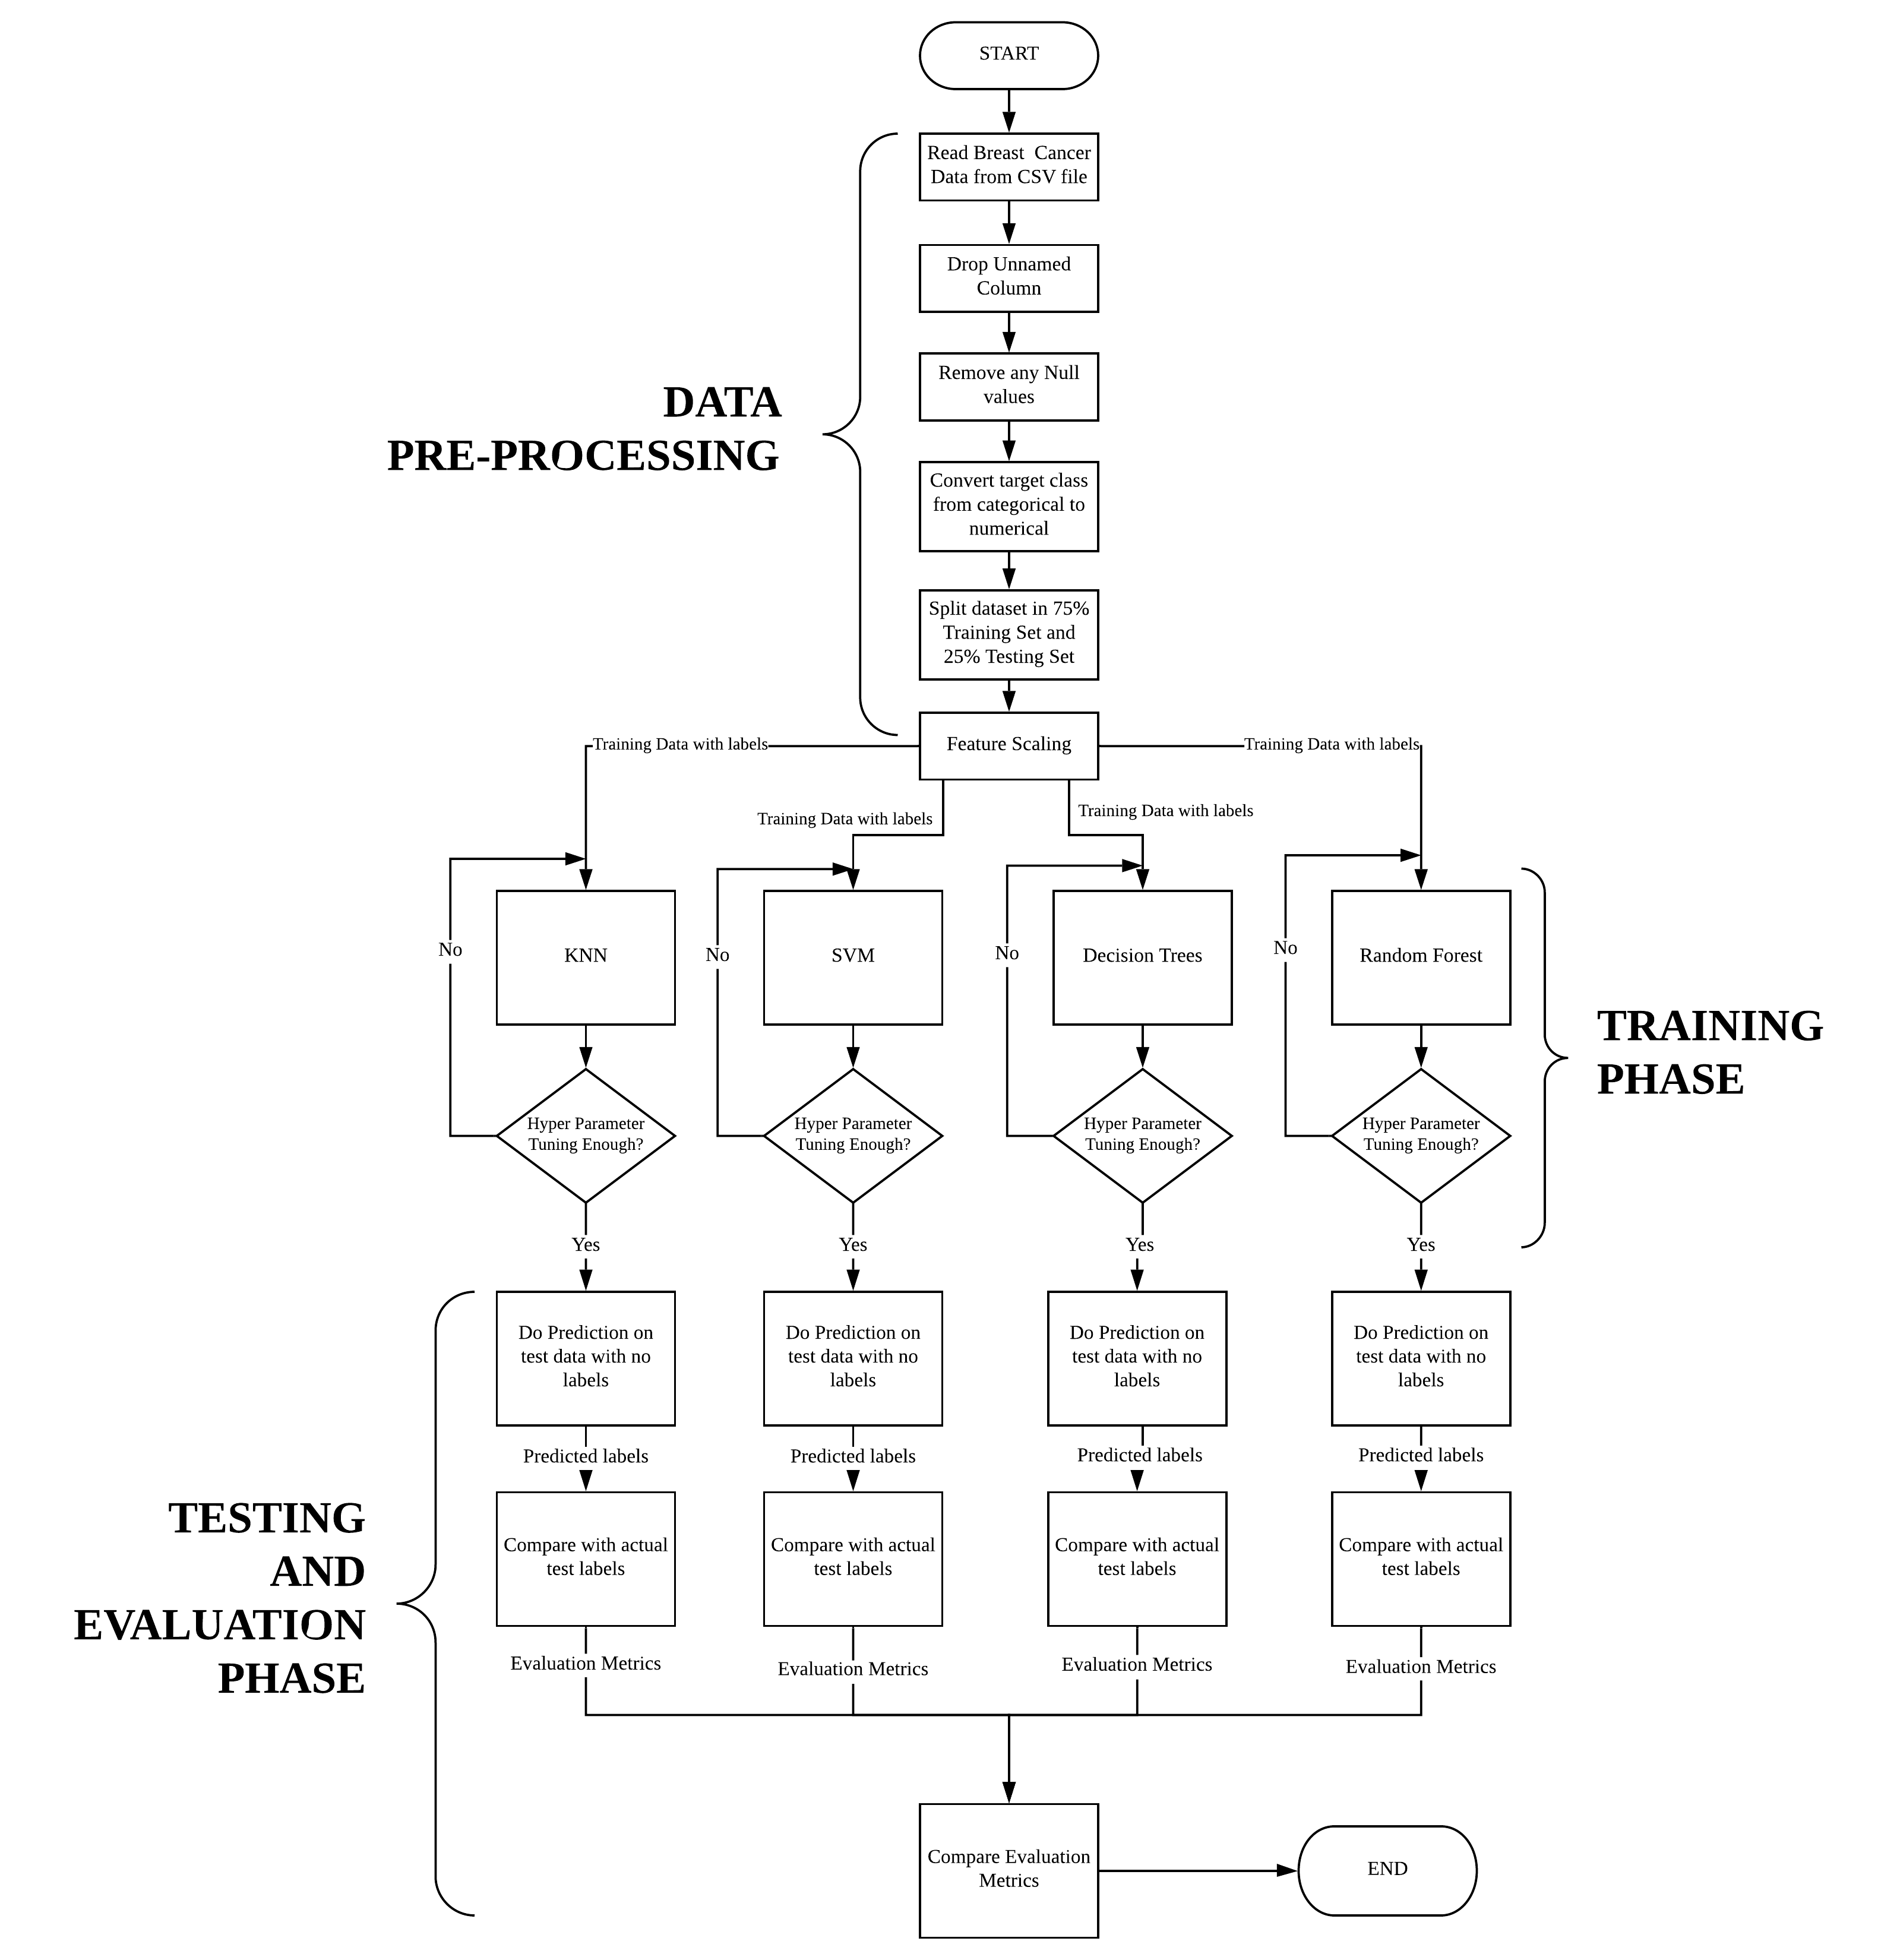
\includegraphics[scale = 0.73]{methodology.png}
   \caption{Flowchart showing the method used for classification}
   \label{Fig:mtd}
\end{figure*}

\subsection{Dataset}
The dataset used in this research is accessible to the public and was developed by Dr. William H. Wolberg, a physician at the University of Wisconsin Hospital in Madison, Wisconsin, USA. The dataset can be downloaded from the Kaggle website \cite{uci_2016}. Dr. Wolberg used fluid samples from individuals with strong breast masses and an easy-to-use graphical computer program called Xcyt to produce the dataset. Xcyt is capable of analyzing cytological characteristics based on digital scans. It uses a curve-fitting algorithm to calculate ten features from each of the sample cells. After that it calculates the mean value, extreme value, and standard error of each feature for the image, returning a real-valued vector of 30. The ten features calculated are:

\begin{enumerate}
  \item radius (mean of distances from center to points on the perimeter)
  \item texture (standard deviation of gray-scale values)
  \item perimeter
  \item area
  \item smoothness (local variation in radius lengths)
  \item compactness 
  \item concavity (severity of concave portions of the contour)
  \item concave points (number of concave portions of the contour)
  \item symmetry
  \item fractal dimension (“coastline approximation” — 1)\\
\end{enumerate} 

The dataset also contains an id column which basically represents individual patients. There is a diagnosis column which represents if the patient has breast cancer or not. Values of "M" representing malignant and "B" representing benign are used in the diagnosis column. The class distribution is 357 benign patients and 212 malignant patients. In summary, the dataset contains 32 columns and 569 rows where out of the 32 columns, there are 30 feature columns, 1 patient id column and lastly the diagnosis column which is basically the target class used for classification.
 
\subsection{Data Preprocessing}

The dataset is first read from the csv file as a data frame using the panda's library. An unnamed column is automatically added when reading the file, so it is removed using the "drop" command. Then the dataset is checked for any missing or null values. There were no missing values in this dataset. The target column in this dataset is categorical having the values "M" and "B". This represents a tumor being either malignant (cancerous tumor) or benign (non-cancerous tumor). As the inputs for machine learning algorithms are expected to be numerical, the categorical values for the diagnosis column are assigned the values 1 and 0 where 1 represents "M" and 0 represents "B" using the "LabelEncoder" library of scikit learn. To split the dataset for training and testing, scikit learn's "train\_test\_split" function is used. The dataset was split into 75\% for training and 25\% for testing.\\

Scaling is done next to bring the data in the feature columns of both the training and test sets onto a common scale. After inspecting the data, it is seen that the values in feature columns vary a lot. For example the mean of the column named "area\_mean" is 654 and the mean of the column named "compactness\_mean" is 0.1. But since, most of the machine learning algorithms use Euclidean distance between two data points in their computations, we need to bring all features to the same level of magnitude. To do this, scikit learn's "StandardScaler" library is used \cite{scaler}. The math equations that this library uses are shown below:

\begin{equation}
\label{eqn:standardization}
\textrm{Standardization: }
z = \frac{x - \mu}{\sigma}
\end{equation}

\begin{equation}
\label{eqn:mean}
\textrm{with Mean: }
\mu = \frac{1}{N} \sum\limits_{i=1}^N (x_i) 
\end{equation}

\begin{equation}
\label{eqn:std}
\textrm{and Standard Deviation: }
\sigma = \sqrt{\frac{1}{N} \sum\limits_{i=1}^N(x_i - \mu)^2}
\end{equation}

The idea behind "StandardScaler" is that it will transform the data such that its distribution will have a mean value of zero and standard deviation of one using equations \ref{eqn:mean} and \ref{eqn:std} . Given the distribution of the data, each value in the dataset will have the sample mean value subtracted, and then divided by the standard deviation of the whole dataset using the equation \ref{eqn:standardization}.


\subsection{Training Phase}

After the data-preprocessing step is finished, the training set is used to train different machine learning algorithms. The following subsections show how different machine learning algorithm works and how the hyper parameters of each algorithm were tuned to achieve better results.\\

\subsubsection{K-Nearest Neighbours (KNN)}

KNN is a machine learning algorithm that can be used for both classification and regression. For the purpose of this research, KNN is used as a classification technique. The principle behind nearest neighbor methods is to find a predefined number of training samples closest in distance to the new point, and predict the label from these \cite{knn}. The number of samples can be a user-defined constant (k-nearest neighbor learning), or vary based on the local density of points (radius-based neighbor learning). The distance can, in general, be any metric measure: standard Euclidean distance and Minkowski distance are the most common choices. Despite its simplicity, nearest neighbors has been successful in a large number of classification and regression problems, including handwritten digits and satellite image scenes. Scikit learn has a library function called "KNeighborsClassifier"  for using this algorithm \cite{knn_scikit}. The hyper parameters that are avaialble to use for this function are:

\begin{itemize}
  \item \textbf{n\_neighbors:} number of neighbours to be taken into consideration for the voting process.
  \item \textbf{p:} power parameter for the Minkowski metric. When p = 1, this is equivalent to using manhattan distance (l1). For p = 2, it is equivalent to using euclidean distance (l2). For arbitrary p, minkowski distance (l\_p) is used. Equation \ref{eqn:m1} and  \ref{eqn:m2} below shows how Minkowski distance is calculated:\\
  
\end{itemize}

The Minkowski distance of order p between two points

\begin{equation}
\label{eqn:m1}
X = (x_1, x_2,....,x_n) \textrm{ and } Y = (y_1, y_2,....,y_n)
\end{equation}

is defined as
\begin{equation}
\label{eqn:m2}
D(X,Y) = (\sum\limits_{i=1}^N |x_i - y _i|^p)^\frac{1}{p}
\end{equation}

Firstly, "n\_neighbors" parameter tuning was performed. AUC curve was plotted for different values of "n\_neighbors" for both the training and testing set. As shown in figure \ref{Fig:knnNeighbor}, AUC score for the testing data (red line) is highest when the neighbour value is 15. So the optimal neighbour value is 15. Keeping "n\_neighbors" at a constant value of 15,  "p" parameter tuning was performed. An AUC curve was plotted for different values of "p" for both the training and testing set. As shown in figure \ref{Fig:knnp}, AUC score for the testing data (red line) is highest when the p value is 2. Final parameter values for "n\_neighbors" and "p" are 15 and 2 respectively. For "n\_neighbors" tuning, integer values between 1 and 30 were tested. For "p" tuning, integer values between 1 and 5 were tested. 

\begin{figure}[H]
	\centering
	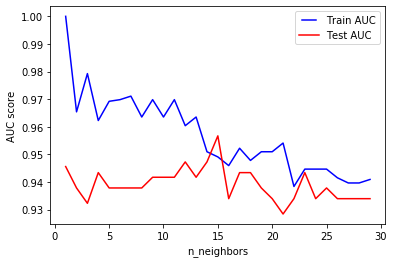
\includegraphics[width=\linewidth]{neighboursTune_KNN.png}
	\caption{n\_neighbour parameter tuning (KNN)}
	\label{Fig:knnNeighbor}
\end{figure}

\begin{figure}[H]
	\centering
	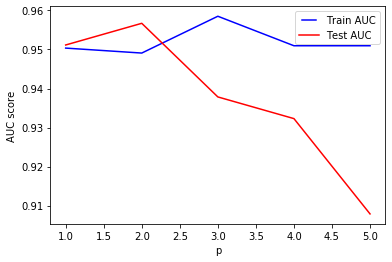
\includegraphics[width=\linewidth]{pTune_KNN.png}
	\caption{p parameter tuning (KNN)}
	\label{Fig:knnp}
\end{figure}


 \subsubsection{Decision Trees (DT)}
Decision tree learning is the construction of a decision tree from class-labeled training tuples. A decision tree is a flow-chart-like structure, where each internal (non-leaf) node denotes a test on an attribute, each branch represents the outcome of a test, and each leaf (or terminal) node holds a class label. The topmost node in a tree is the root node.  Decision tree generation consists of two phases: 1) Tree construction and 2) Tree Pruning. In the first phase, all the training examples are at the root. Examples are partitioned recursively based on selected attributes. This partition is done by choosing a variable at each step that best splits the set of examples. Different algorithms use different metrics for measuring "best". These algorithms generally measure the homogeneity of the target variable within the subsets. In the second phase, tree branches that reflect noise or outliers are identified and removed. Scikit learn has a library function called "DecisionTreeClassifier"  for using this algorithm \cite{dtree}. The hyper parameters that are avaialble to use for this function are:

\begin{itemize}
  \item \textbf{max\_depth:} indicates how deep the tree can be.
  \item \textbf{min\_samples\_split:} represents the minimum number of samples required to split an internal node.
  \item \textbf{max\_features:} represents the number of features to consider when looking for the best split.
\end{itemize}

Firstly, "max\_depth" parameter tuning was performed. An AUC curve was plotted for different values of "max\_depth" for both the training and testing set. As shown in figure \ref{Fig:dt1}, AUC score for the testing data is highest when "max\_depth" is equal to 4. So "max\_depth" value of 4 is selected as optimal. Keeping  "max\_depth"  at a constant value of 4,  "min\_samples\_split" parameter tuning was performed. An AUC curve was plotted for different values of "min\_samples\_split" for both the training and testing set. As shown in figure \ref{Fig:dt2}, AUC score for the testing data is highest when "min\_samples\_split"  is equal to 0.05. So "min\_samples\_split"  value of 0.05 is selected as optimal.\\

Keeping  "max\_depth"  and  "min\_samples\_split"  at a constant value of 4 and 0.05,  "max\_features" parameter tuning was performed. An AUC curve was plotted for different values of "max\_features"  for both the training and testing set. As shown in figure \ref{Fig:dt3}, AUC score for the testing data is highest when "max\_features" is equal to 15. So "max\_features"  value of 15 is selected as optimal. Final parameter values for "max\_depth", "min\_samples\_split" and  "max\_features"  are 4, 0.05 and 15 respectively. For "max\_depth" tuning, integer values between 1 and 32 were tested. For  "min\_samples\_split" tuning, decimal values between 0.1 and 1.0 were tested to represent 10\% to 100\% of the samples. For "max\_features" tuning, integer values between 1 and 30 were tested.

\begin{figure}[htbp]
	\centering
	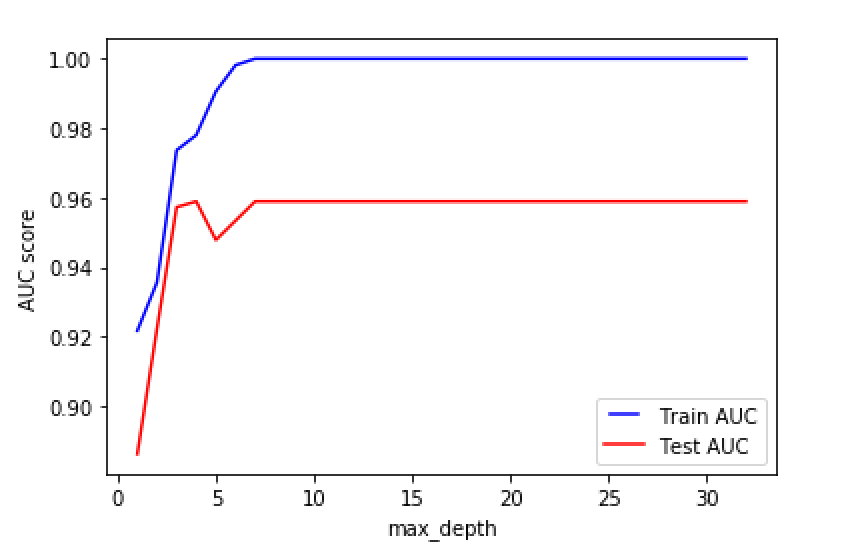
\includegraphics[width=\linewidth]{maxDepth_DT.png}
	\caption{max\_depth parameter tuning (DT)}
	\label{Fig:dt1}
\end{figure}

\begin{figure}[htbp]
	\centering
	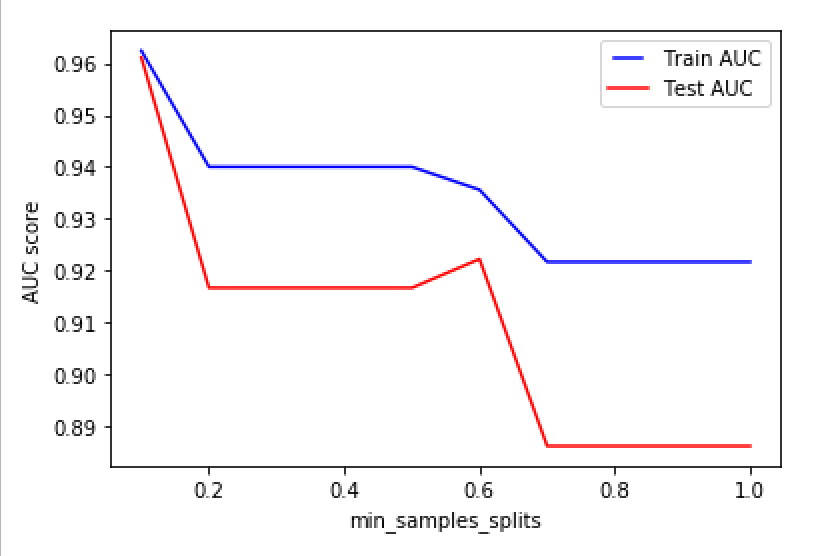
\includegraphics[width=\linewidth]{minSsplit_DT.png}
	\caption{min\_samples\_split parameter tuning (DT)}
	\label{Fig:dt2}
\end{figure}

\begin{figure}[H]
	\centering
	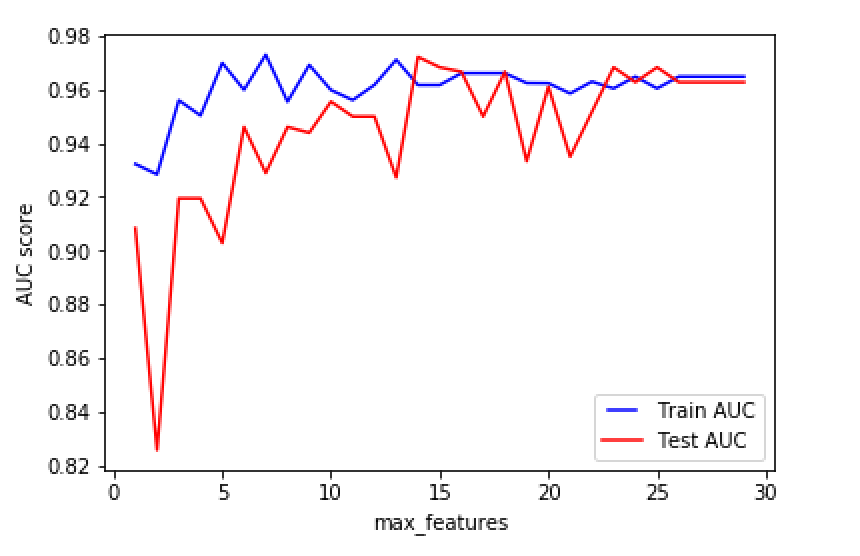
\includegraphics[width=\linewidth]{maxFeatures_DT.png}
	\caption{max\_features parameter tuning (DT)}
	\label{Fig:dt3}
\end{figure}



 \subsubsection{Random Forests (RF)}
 
Random forests or random decision forests are an ensemble learning method for classification, regression and other tasks that operates by constructing a multitude of decision trees at training time and outputting the class that is the mode of the classes (classification) or mean prediction (regression) of the individual trees. Random decision forests correct for decision trees' habit of overfitting to their training set. In this research, random forests is used for classification. Scikit learn has a library function called "RandomForestClassifier" for using this algorithm \cite{rforest}. The hyper parameters that are avaialble to use for this function are:

\begin{itemize}
  \item \textbf{N\_estimators:} represents the number of trees in the forest
  \item \textbf{max\_depth:}  represents the depth of each tree in the forest.
  \item \textbf{max\_features:} represents the number of features to consider when looking for the best split.\\
\end{itemize}

Firstly, "N\_estimators" parameter tuning was performed. An AUC curve was plotted for different values of "N\_estimators" for both the training and testing set. As shown in figure \ref{Fig:rf1}, it can be seen that the test accuracy is highest when "N\_estimators" is equal to 10. So the "N\_estimators" value of 10 is selected as optimal. Keeping  "N\_estimators"  at a constant value of 10,  "max\_depth" parameter tuning was performed. An AUC curve was plotted for different values of "max\_depth" for both the training and testing set. As shown in figure \ref{Fig:rf2}, it can be seen that the test accuracy is highest when "max\_depth" is equal to 5. So the "max\_depth" value of 5 is selected as optimal. Keeping  "N\_estimators"  and "max\_depth" at a constant value of 10 and 5 respectively,  "max\_features" parameter tuning was performed. An AUC curve was plotted for different values of "max\_features" for both the training and testing set. As shown in figure \ref{Fig:rf3}, it can be seen that the test accuracy is highest when "max\_features" is equal to 27. So the ""max\_features" value of 27 is selected as optimal. Final parameter values for  "N\_estimators", "max\_depth" and  "max\_features"  are 10, 5 and 27 respectively. For "N\_estimators" tuning, integer values tested are \[1, 2, 4, 8, 16, 32, 64, 100, 200\]For  "max\_depth" tuning, integer values between 1 and 32 were tested. For "max\_features" tuning, integer values between 1 and 30 were tested.


\begin{figure}[htbp]
	\centering
	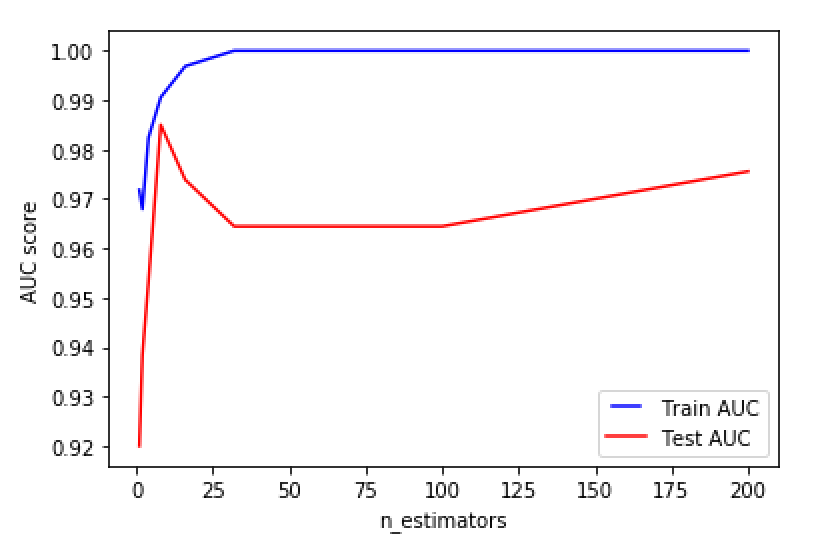
\includegraphics[width=\linewidth]{nestimator_RF.png}
	\caption{n\_estimators parameter tuning (RF)}
	\label{Fig:rf1}
\end{figure}
 
\begin{figure}[htbp]
	\centering
	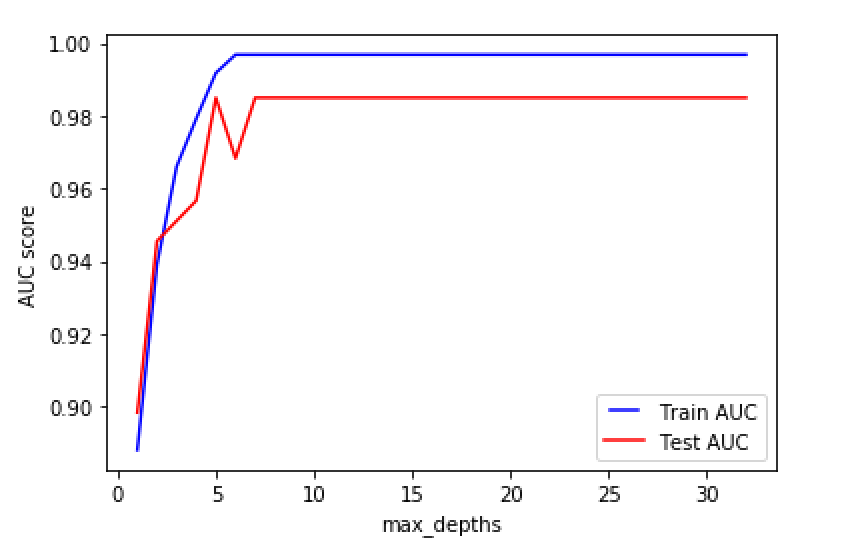
\includegraphics[width=\linewidth]{maxDepth_RF.png}
	\caption{max\_depth parameter tuning (RF)}
	\label{Fig:rf2}
\end{figure}

\begin{figure}[H]
	\centering
	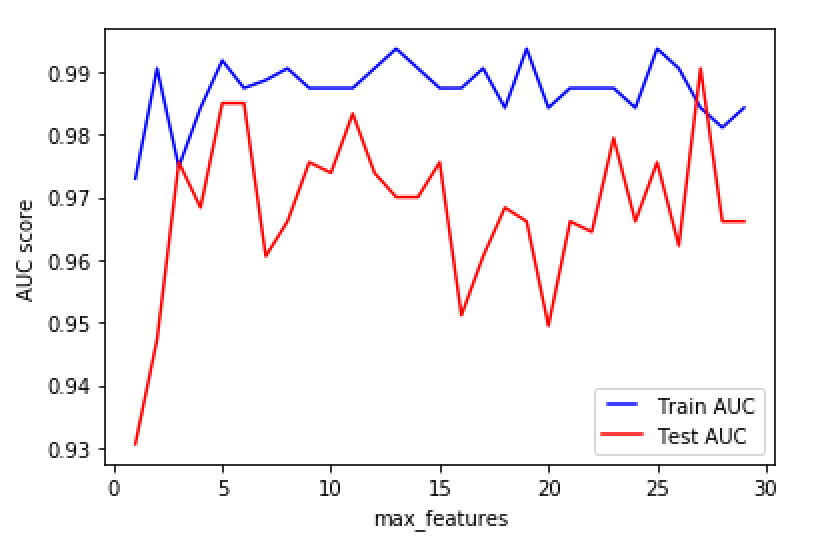
\includegraphics[width=\linewidth]{maxFeatures_RF.png}
	\caption{max\_features parameter tuning (RF)}
	\label{Fig:rf3}
\end{figure}


\subsubsection{Support Vector Machines (SVM)}
A support-vector machine constructs a hyperplane or set of hyperplanes in a high- or infinite-dimensional space, which can be used for classification, regression, or other tasks like outliers detection. Given a set of training examples, each marked as belonging to one or the other of two categories, a SVM training algorithm builds a model that assigns new examples to one category or the other. A SVM model is a representation of the examples as points in space, mapped so that the examples of the separate categories are divided by a clear gap that is as wide as possible. New examples are then mapped into that same space and predicted to belong to a category based on the side of the gap on which they fall. Scikit learn has a library function called "SVC" for using this algorithm \cite{SVM}. The hyper parameters that are avaialble to use for this function are:\\

\begin{itemize}
  \item \textbf{C:} is the penalty parameter of the error term. It controls the trade off between smooth decision boundary and classifying the training points correctly.
  \item \textbf{gamma:}  is a parameter for non linear hyperplanes. The higher the gamma value, the more it tries to exactly fit the training data set.
  \item \textbf{kernel:} selects the type of hyperplane used to separate the data. Using ‘linear’ will use a linear hyperplane (a line in the case of 2D data). ‘rbf’ and ‘poly’ uses a non linear hyper-plane\\
\end{itemize}

As there are many possible combinations of parameters for SVM, writing code manually would be a time consuming process. Using the scikit learns "GridSearchCV", it is possible to do all combinations of parameter values provided and the best parameter combination can easily be found. The "GridSearchCV" function needs input of values of the parameters that it needs to test. Firstly, "C" parameter values that are given to the "GridSearchCV" function are 0.001, 0.01, 0.1, 1, and 10. Secondly, "gamma" parameter values that are given to the "GridSearchCV" function are 0.001, 0.01, 0.1, and 1. Finally, "kernel" parameter values that are given to the "GridSearchCV" function are "linear", "rbf" and "poly". The best combination of parameter values given by the GridSearchCV were 0.1, 0.001 and linear for "C", "gamma" and "kernel" respectively.

\section{Results and Discussion}

Each of the trained models were tested with the same test data. Different evaluation metrics were extracted from each of the trained models. Evaluation metrics that were used were:\\

 \begin{itemize}
  \item \textbf{True Positive (TP):} number of times  both the actual and the predicted class values are "malignant".
  \item \textbf{False Positive (FP):} number of times the actual class is "malignant" and the predicted class is "benign".
  \item \textbf{True Negative: (TN)} number of times both the actual and the predicted class values are "benign".
  \item \textbf{False Negative (FN):} number of times the actual class is "benign" and the predicted class is "malignant".
  \item \textbf{Precision:} when the model predicts the class value to be "malignant", how many times is it correct?. Calculated using the formula $TP/(TP + FP)$
  \item \textbf{Recall:} when the actual class value is "malignant", how many times does the model predict the class to also be "malignant"? Calculated using the formula $TP/(TP + FN)$
  \item \textbf{Accuracy:} number of correct predictions by the model from the total number of test data. Calculated using the formula $(TP + TN) /(TP + FP + FN + TN)$\\
\end{itemize}

\begin{table}[htbp]
\centering
\setlength{\tabcolsep}{6pt}
\renewcommand{\arraystretch}{2}
\begin{tabular}{|l|l|l|l|l|}
\hline
                                          & \textbf{KNN} & \textbf{DT} & \textbf{SVM} & \textbf{RF} \\ \hline
\textbf{Accuracy before parameter tuning} & 0.950        & 0.880       & 0.90         & 0.972       \\ \hline
\textbf{Accuracy after parameter tuning}  & 0.965        & 0.965       & 0.965        & 0.993       \\ \hline
\end{tabular}
\caption{Accuracy of classifiers before and after tuning}
\label{table:1}
\end{table}

\begin{table}[htbp]
\centering
\setlength{\tabcolsep}{15pt}
\renewcommand{\arraystretch}{2}
\begin{tabular}{|l|l|l|l|l|}
\hline
                   & \textbf{KNN} & \textbf{DT} & \textbf{SVM} & \textbf{RF} \\ \hline
\textbf{TP}        & 49           & 52          & 50           & 52          \\ \hline
\textbf{FP}        & 1            & 4           & 2            & 0           \\ \hline
\textbf{TN}        & 9            & 86          & 88           & 90          \\ \hline
\textbf{FN}        & 4            & 1           & 3            & 1           \\ \hline
\textbf{Precision} & 0.98         & 0.93        & 0.96         & 1           \\ \hline
\textbf{Recall}    & 0.92         & 0.98        & 0.94         & 0.98        \\ \hline
\end{tabular}
\caption{Comparison of Fine-Tuned Classifiers using Evaluation metrics}
\label{table:2}
\end{table}

All the evaluation metrics were recorded in both TABLE \ref{table:1} and TABLE \ref{table:2}. In terms of improvement of accuracy before and after parameter tuning, from TABLE \ref{table:1} it can be seen that decision trees have the highest accuracy improvement of 8.5\%. In terms of precision, from TABLE \ref{table:2} it can be seen that all of the models were able to give very good results($>=0.93$). Among them random forest was able to perform best with a perfect precision score of 1. KNN had the second best precision score with a value of 0.98. In terms of recall, from TABLE \ref{table:2} it can be seen that all of the models were again able to give very good results($>=0.92$). Among them random forest and decision trees were tied with a near perfect recall score of 0.98. In terms of accuracy of models after fine tuning, from TABLE \ref{table:1} it can be seen that random forest was able to perform best with a near perfect accuracy score of 0.993. KNN, Decision trees and SVM were second best with an accuracy score of 0.965. In terms of time taken for parameter tuning, KNN took the least time. As there is only one parameter that had to be tuned for KNN (neighbors parameter) compared to 3 parameters for the other three, it took lesser time to find the optimal parameter for KNN.\\

It is easier to analyze why random forests provides better results compared to decision trees \cite{adv}. There are two reasons mainly. Firstly, there is a reduction in overfitting by averaging several trees. Secondly, there is less variance using multiple trees. This means the chance of stumbling across a classifier that doesn’t perform well because of the relationship between the train and test data is less when using multiple trees. Performance of KNN and SVM depend heavily on the dataset itself. To further improve the accuracy of both KNN and SVM, the dataset needs to be studied further to see how separable the data points are in different dimensional space.


\section{Conclusion}
With the improvements in machine learning tools, the effects of these innovations are entering to more application domains day-by-day and medical field is one of them. Decision making in medical field can be a trouble sometimes. Classification systems that are used in medical decision making provide medical data to be examined in shorter time and more detailed. According to the statistical data for breast cancer in the world, this disease is among the most prevalent cancer types. In the same time, this cancer type is also among the most curable ones if it can be diagnosed early. In this study, for the diagnosis of breast cancer, different machine learning classification algorithms were compared on how well they could classify unseen breast cancer data. Among the classification algorithms, random forest was able to provide the best results with an accuracy of 99.3\%. The results strongly suggest that random forest can aid in the diagnosis of breast cancer. This research also has some limitations. Firstly, the splitting statergy used for getting the training and test data could be bias. It could be possible that a classifier that performs well on some specific test set may not perform that well on other test sets. So it would be better to remove this bias by using K-fold cross validation technique. Another limitation is that the hyper-parameter that were selected as optimal may only be a local optimal compared to being a global optimal because of the fact that the ranges that were used to test each hyper-parameter were defined manually. For future research, I would like to focus on using K-fold cross validation technique for testing my classification models and also use more advanced hyper-parameter tuning strategies. Furthermore, the use of other classification algorithms like neural networks can also be explored in classifying breast cancer. 


% if have a single appendix:
%\appendix[Proof of the Zonklar Equations]
% or
%\appendix  % for no appendix heading
% do not use \section anymore after \appendix, only \section*
% is possibly needed

% use appendices with more than one appendix
% then use \section to start each appendix
% you must declare a \section before using any
% \subsection or using \label (\appendices by itself
% starts a section numbered zero.)
%
\bibliographystyle{IEEEtran}

% argument is your BibTeX string definitions and bibliography database(s)
\bibliography{ref}{}


% use section* for acknowledgment

% Can use something like this to put references on a page
% by themselves when using endfloat and the captionsoff option.
\ifCLASSOPTIONcaptionsoff
  \newpage
\fi



% trigger a \newpage just before the given reference
% number - used to balance the columns on the last page
% adjust value as needed - may need to be readjusted if
% the document is modified later
%\IEEEtriggeratref{8}
% The "triggered" command can be changed if desired:
%\IEEEtriggercmd{\enlargethispage{-5in}}

% references section

% can use a bibliography generated by BibTeX as a .bbl file
% BibTeX documentation can be easily obtained at:
% http://mirror.ctan.org/biblio/bibtex/contrib/doc/
% The IEEEtran BibTeX style support page is at:
% http://www.michaelshell.org/tex/ieeetran/bibtex/

%
% <OR> manually copy in the resultant .bbl file
% set second argument of \begin to the number of references
% (used to reserve space for the reference number labels box)


% biography section
% 
% If you have an EPS/PDF photo (graphicx package needed) extra braces are
% needed around the contents of the optional argument to biography to prevent
% the LaTeX parser from getting confused when it sees the complicated
% \includegraphics command within an optional argument. (You could create
% your own custom macro containing the \includegraphics command to make things
% simpler here.)
%\begin{IEEEbiography}[{\includegraphics[width=1in,height=1.25in,clip,keepaspectratio]{mshell}}]{Michael Shell}
% or if you just want to reserve a space for a photo:



% insert where needed to balance the two columns on the last page with
% biographies
%\newpage



% You can push biographies down or up by placing
% a \vfill before or after them. The appropriate
% use of \vfill depends on what kind of text is
% on the last page and whether or not the columns
% are being equalized.

%\vfill

% Can be used to pull up biographies so that the bottom of the last one
% is flush with the other column.
%\enlargethispage{-5in}



% that's all folks
\end{document}


